
\documentclass[12pt,article]{memoir}

\usepackage{fancyhdr}
\usepackage{graphicx}
\usepackage{fontspec}
\setmainfont{Calibri}
\usepackage{tikz}
\usetikzlibrary{calc}
\usepackage{xcolor}
\usepackage{xpatch}
\usepackage{hyperref}
\usepackage{tabu}
\usepackage{float}
\usepackage[autostyle, english = american]{csquotes}



\usepackage[yyyymmdd]{datetime} % change date format to yyyy/mm/dd to fit ISO8601

\renewcommand{\familydefault}{\sfdefault} % set font
\renewcommand{\dateseparator}{--} % change date-seperators to - to fit ISO8601

\renewcommand\contentsname{Table of Contents}

\chapterstyle{section}
\renewcommand*{\chapnumfont}{\normalfont\HUGE\bfseries\sffamily}
\renewcommand*{\chaptitlefont}{\normalfont\HUGE\bfseries\sffamily}

\makeatletter 
% define macro for itemcode
\newcommand\itemcode[1]{\renewcommand\@itemcode{#1}}
\newcommand\@itemcode{}

% define macro for rev number
\newcommand\revnumber[1]{\renewcommand\@revnumber{#1}}
\newcommand\@revnumber{}
\makeatother

\definecolor{orbitOrange}{RGB}{250,62,0} % the ORBiT orange

\setlrmarginsandblock{2.5cm}{2.5cm}{*}
\setulmarginsandblock{2.5cm}{*}{1}
\checkandfixthelayout 

\setlength{\beforechapskip}{0cm} % reduce chapter spacing

\hypersetup{
    colorlinks,
    citecolor=black,
    filecolor=black,
    linkcolor=black,
    urlcolor=black
}

%**********************************************************************
%Document titles etc. defined here: (replace [] as well)
\title{OA-II VEH Camera System Design}
\author{Jinzhi Cai}
\itemcode{DR00002}
\revnumber{A01}
\date{\today}
%end of document titles etc.
%**********************************************************************

\makeatletter
\let\runtitle\@title
\let\runitemcode\@itemcode
\makeatother

% set header style
\pagestyle{fancy}
{
	\fancyheadoffset{0cm}

	\lhead{\runtitle \ - \runitemcode}
	\rhead{Page: \thepage }
	%\chead{\leftmark} % section name
}

\newcommand{\OrbitBackground}{% For a logo drawn with TikZ
\begin{tikzpicture}[remember picture,overlay] % draw background
	\coordinate (bl) at (current page.south west);
	\coordinate (r) at (current page.east);
    \coordinate (A) at ($(bl)+(0,3cm)$);
    \coordinate (B) at ($(r)+(0,-2cm)$);
    \coordinate (C) at (current page.south east);
    \coordinate (ctrlNode) at ($(current page.south) + (0cm,1cm)$);
    \coordinate (ctrlNode2) at ($(current page.south east) + (-1cm,1cm)$);
    \fill[orbitOrange, fill opacity=0.2]
    (A) .. controls (ctrlNode) and (ctrlNode2) .. (B) -- (C) -- (bl);
    \node [white] at ($(C) + (-3cm,1cm)$) {2015-\the\year \ ORBiT@SU};
\end{tikzpicture}
}

\cfoot{\OrbitBackground}

\begin{document}

\begin{tikzpicture}[remember picture,overlay] % draw background
	\coordinate (bl) at (current page.south west);
	\coordinate (r) at (current page.east);
    \coordinate (A) at ($(bl)+(0,3cm)$);
    \coordinate (B) at ($(r)+(0,-2cm)$);
    \coordinate (C) at (current page.south east);
    \coordinate (ctrlNode) at ($(current page.south) + (0cm,1cm)$);
    \coordinate (ctrlNode2) at ($(current page.south east) + (-1cm,1cm)$);
    \fill[orbitOrange]
    (A) .. controls (ctrlNode) and (ctrlNode2) .. (B) -- (C) -- (bl);
    \node [white] at ($(C) + (-3cm,1cm)$) {2015-\the\year \ ORBiT@SU};
\end{tikzpicture}

\makeatletter
	
\includegraphics[width=\textwidth]{../logo.jpg}\\[4ex]
	\begin{center}
	{\fontsize{50}{60}\selectfont \bfseries  \@title }\\[2ex] 
	{\LARGE  \@itemcode}\\
	\end{center}
	\begin{flushright}
	\vspace*{\fill}
	{\LARGE Rev: \@revnumber}\\[2ex]
	{\large \@author}\\[2ex]
	{\large \@date}\\[20ex]
	\end{flushright}
\makeatother
\thispagestyle{empty}
\newpage

\tableofcontents*
\thispagestyle{fancy}
\newpage

%**********************************************************************
% Everything after this is the main document. Edit below this line,

\chapter{Introduction}
\section{Scope}
This document discuss the current camera technology and construct a design that will fullfill the need for OA-II VEH system.
\section{Purpose}
The goal for this document is come up with a design that will provide four 1080p 60Hz video steam and storage to a central storage media by research the current camera technology.
\chapter{Revision History}

\begin{table}[H]
	\centering
	\resizebox{0.8\textwidth}{!}{%
		\begin{tabu}{r || c | c | c }
		Rev\# & Editor & Delta & Date\\ \hline
		A01 & Jinzhi Cai & Initialize & 2019-7-10\\
		\end{tabu}
	}
	\caption{Summary of Revision History}
	\label{tab:edatools}
\end{table}

\newpage
\chapter{General Structure of Camera System}
\section{Introduction}
The most basic camera system have three part. The camera sensor is the device that will receive data from the environment and transfer it via the camera interface. The data that flow out from the sensor is call raw data. It contain all the information that the camera get from the environment. A 1080p 60Hz camera have $1920*1080=2073600 pixels$. One pixels usually take $3 Bytes$ to save. For each second, $2073600*3*60=373248000Bytes$ will be created. That will be $355.96MB/s$ for one single camera.The encoder is use to compress the video steam smaller for it to transmission via long distence data link(usually with in $1MB/s$). The storage unit is use to save the video steam to a file and allow future replay.
\begin{figure}[htp]
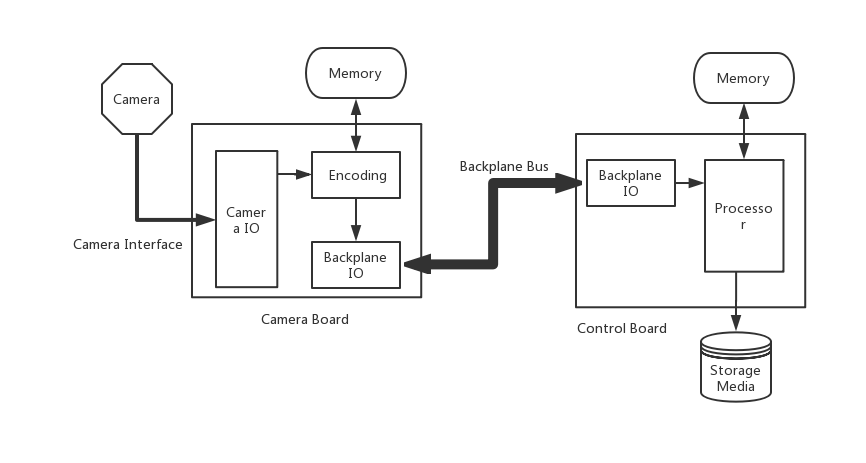
\includegraphics[width=\textwidth]{DR00002_GenDia.png}
 \caption{General Structure of Camera System}	
\end{figure}
\newpage
%
%**********************************************************************
\chapter{Camera Sensor and Relative Interface}
\section{Introduction}
The camera sensor is the most improtant part in the camera system. Modern camera sensor usually use one of those three camera interface.
\section{DVP Interface} 
\begin{figure}[htp]
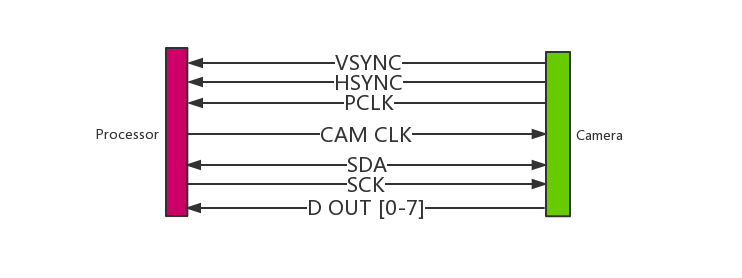
\includegraphics[width=\textwidth]{DR00002_DVP.png}
 \caption{Physical Layer for DVP Interface}	
\end{figure}
\section{LVDS Interface}
\begin{figure}[htp]
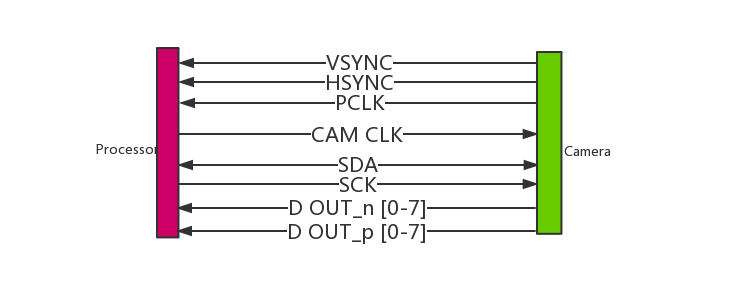
\includegraphics[width=\textwidth]{DR00002_LVDS.png}
 \caption{Physical Layer for LVDS Interface}	
\end{figure}
\section{MIPI CSI-2 Interface}
\begin{figure}[htp]
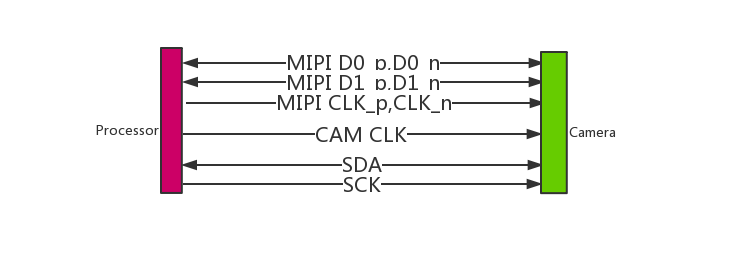
\includegraphics[width=\textwidth]{DR00002_MIPI.png}
 \caption{Physical Layer for MIPI Interface}	
\end{figure}
\newpage
%**********************************************************************
\chapter{H.264 Video Steam Encoding}
\section{Introduction}
\section{IP core Description}
\newpage
%**********************************************************************
\chapter{File System and Video Storage}
\newpage
%**********************************************************************
\chapter{System Diagram}
\newpage
%end of document
%**********************************************************************
\end{document}